% Options for packages loaded elsewhere
\PassOptionsToPackage{unicode}{hyperref}
\PassOptionsToPackage{hyphens}{url}
%
\documentclass[
]{article}
\usepackage{amsmath,amssymb}
\usepackage{lmodern}
\usepackage{ifxetex,ifluatex}
\ifnum 0\ifxetex 1\fi\ifluatex 1\fi=0 % if pdftex
  \usepackage[T1]{fontenc}
  \usepackage[utf8]{inputenc}
  \usepackage{textcomp} % provide euro and other symbols
\else % if luatex or xetex
  \usepackage{unicode-math}
  \defaultfontfeatures{Scale=MatchLowercase}
  \defaultfontfeatures[\rmfamily]{Ligatures=TeX,Scale=1}
\fi
% Use upquote if available, for straight quotes in verbatim environments
\IfFileExists{upquote.sty}{\usepackage{upquote}}{}
\IfFileExists{microtype.sty}{% use microtype if available
  \usepackage[]{microtype}
  \UseMicrotypeSet[protrusion]{basicmath} % disable protrusion for tt fonts
}{}
\makeatletter
\@ifundefined{KOMAClassName}{% if non-KOMA class
  \IfFileExists{parskip.sty}{%
    \usepackage{parskip}
  }{% else
    \setlength{\parindent}{0pt}
    \setlength{\parskip}{6pt plus 2pt minus 1pt}}
}{% if KOMA class
  \KOMAoptions{parskip=half}}
\makeatother
\usepackage{xcolor}
\IfFileExists{xurl.sty}{\usepackage{xurl}}{} % add URL line breaks if available
\IfFileExists{bookmark.sty}{\usepackage{bookmark}}{\usepackage{hyperref}}
\hypersetup{
  pdftitle={Analysis of the total number of family members},
  pdfauthor={Group\_01},
  hidelinks,
  pdfcreator={LaTeX via pandoc}}
\urlstyle{same} % disable monospaced font for URLs
\usepackage[margin=1in]{geometry}
\usepackage{longtable,booktabs,array}
\usepackage{calc} % for calculating minipage widths
% Correct order of tables after \paragraph or \subparagraph
\usepackage{etoolbox}
\makeatletter
\patchcmd\longtable{\par}{\if@noskipsec\mbox{}\fi\par}{}{}
\makeatother
% Allow footnotes in longtable head/foot
\IfFileExists{footnotehyper.sty}{\usepackage{footnotehyper}}{\usepackage{footnote}}
\makesavenoteenv{longtable}
\usepackage{graphicx}
\makeatletter
\def\maxwidth{\ifdim\Gin@nat@width>\linewidth\linewidth\else\Gin@nat@width\fi}
\def\maxheight{\ifdim\Gin@nat@height>\textheight\textheight\else\Gin@nat@height\fi}
\makeatother
% Scale images if necessary, so that they will not overflow the page
% margins by default, and it is still possible to overwrite the defaults
% using explicit options in \includegraphics[width, height, ...]{}
\setkeys{Gin}{width=\maxwidth,height=\maxheight,keepaspectratio}
% Set default figure placement to htbp
\makeatletter
\def\fps@figure{htbp}
\makeatother
\setlength{\emergencystretch}{3em} % prevent overfull lines
\providecommand{\tightlist}{%
  \setlength{\itemsep}{0pt}\setlength{\parskip}{0pt}}
\setcounter{secnumdepth}{-\maxdimen} % remove section numbering
\usepackage{booktabs}
\usepackage{longtable}
\usepackage{array}
\usepackage{multirow}
\usepackage{wrapfig}
\usepackage{float}
\usepackage{colortbl}
\usepackage{pdflscape}
\usepackage{tabu}
\usepackage{threeparttable}
\usepackage{threeparttablex}
\usepackage[normalem]{ulem}
\usepackage{makecell}
\usepackage{xcolor}
\ifluatex
  \usepackage{selnolig}  % disable illegal ligatures
\fi

\title{Analysis of the total number of family members}
\author{Group\_01}
\date{}

\begin{document}
\maketitle

\hypertarget{sec:Intro}{%
\section{Introduction}\label{sec:Intro}}

Data come from the FIES (Family Income and Expenditure Survey) recorded
in the Philippines. The survey, which is undertaken every three years,
is aimed at providing data on family income and expenditure. The data
obtained from this survey are from different regions across the
Philippines. This report will focus on one individual area, the
Cordillera Administrative Region and so region has been removed from the
dataset as it will not be informative as an explanatory variable.

The report will investigate which household related variables influence
the number of people living in a household. The data used consists of
1725 observations of ten variables, two of which are categorical and the
remaining are numerical.

\hypertarget{sec:EDA}{%
\section{Exploratory Data Analysis}\label{sec:EDA}}

Figure 1 shows the distribution of the response variable: Number of
members in a household (variable name
``Total.number.of.family.members''). The modal response is 4 members and
the distribution is right-skewed,

\begin{figure}[H]

{\centering 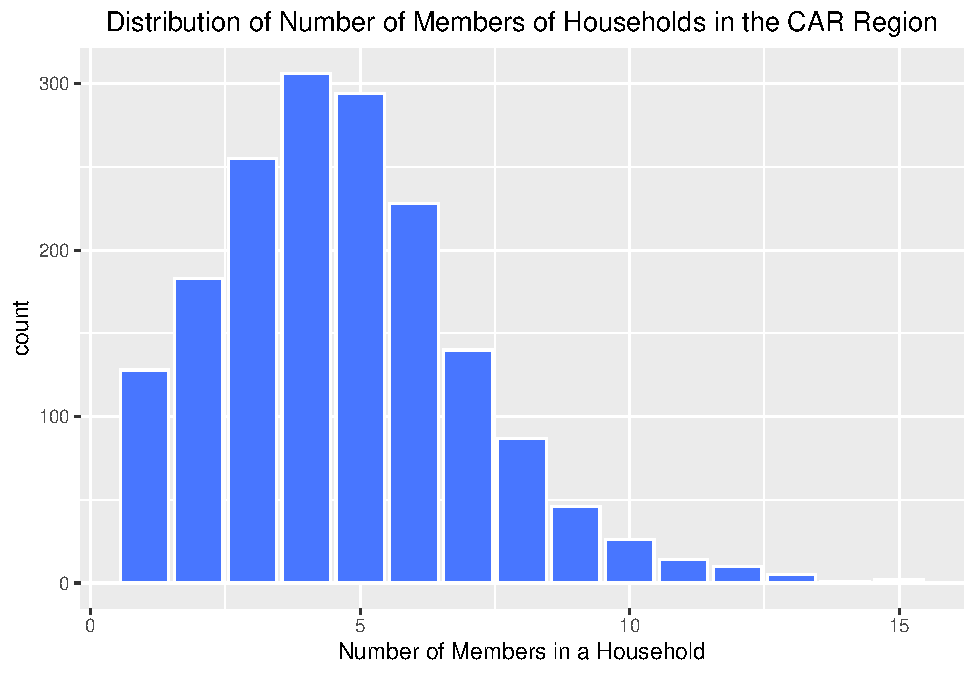
\includegraphics[width=0.8\linewidth]{Group_01_files/figure-latex/distribution of response variable-1} 

}

\caption{Distribution of Response Variable}\label{fig:distribution of response variable}
\end{figure}

The summary below shows the count data for each level of the response
variable and the percentage of total households in the region in each
group.

Figure 2 shows a graphical visualisation for all the variables in the
data set.

\begin{figure}[H]

{\centering 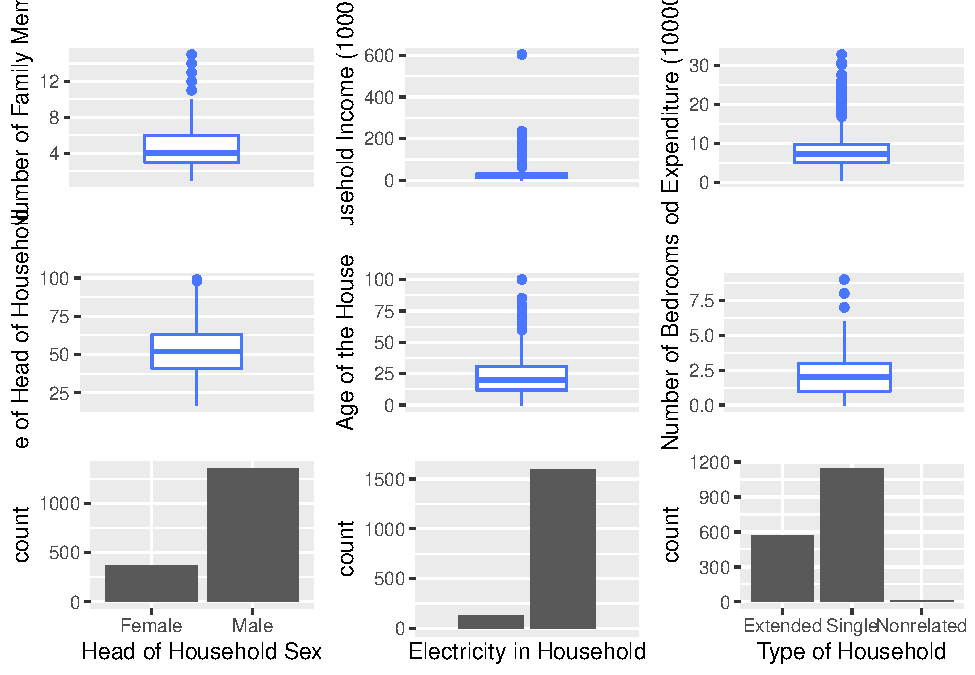
\includegraphics[width=0.8\linewidth]{Group_01_files/figure-latex/all summaries-1} 

}

\caption{Graphical Summaries of Variables}\label{fig:all summaries}
\end{figure}

Table 1 shows summary data for all the numerical variables.There is no
missing data within these variables and so no values will need to be
imputed for the analysis in the report. The response variable, total
number of family members in a household, ranges from 1 to 15, with the
middle 50\% of number of family members falling between 3 and 6 also an
average number of family members of 4.67. There appear to be possible
outliers at the maximum values of Total Household Income and House Floor
Area. The total household income is range from 11988 to 6042860
Philippine Peso. The middle 50\% of total household income is between
118565 and 328335, with an income of 269540.48 peso on average. The
third variable is total food expenditure, in Phillipine peso, which is
the range of 6781 to 327724, with the middle 50\% lies between 51922 and
98493. Then, the household head's age is range from 17 to 99 years, with
the middle 50\% falling between 41 and 63 years of age. Next, the house
floor area is range from 5 to 900 square metres. The central 50\% of the
variable house floor area is between 32 and 102 with an average area of
90.92. The sixth explanatory variable is the house (building) age and it
ranges in value from 0 to 100, with the middle 50\% falling between 12
and 31. The number of bedrooms in the house ranges from 0 to 9 with a
mean average number of bedrooms of 2.26 per household. Finally, we may
look at the binary variable electricity, which denotes whether the
property has electricity access or not, the average score of electricity
is 0.93, which means 93\% household have electricity.

\begin{table}

\caption{\label{tab:numerical summaries}Summary statistics of numerical variables}
\centering
\resizebox{\linewidth}{!}{
\fontsize{10}{12}\selectfont
\begin{tabular}[t]{lrrrrrrrrr}
\toprule
Variable & Missing & Complete & Mean & SD & Min. & 1st Q. & Median & 3rd Q. & Max.\\
\midrule
Total.Number.of.Family.members & 0 & 1 & 4.67 & 2.33 & 1.00 & 3.00 & 4.00 & 6.00 & 15.00\\
Total.Household.Income & 0 & 1 & 26.95 & 27.46 & 1.20 & 11.86 & 18.86 & 32.83 & 604.29\\
Total.Food.Expenditure & 0 & 1 & 8.04 & 4.12 & 0.68 & 5.19 & 7.36 & 9.85 & 32.77\\
Household.Head.Age & 0 & 1 & 52.23 & 14.52 & 17.00 & 41.00 & 52.00 & 63.00 & 99.00\\
House.Floor.Area & 0 & 1 & 90.92 & 99.20 & 5.00 & 32.00 & 54.00 & 102.00 & 900.00\\
\addlinespace
House.Age & 0 & 1 & 22.98 & 15.32 & 0.00 & 12.00 & 20.00 & 31.00 & 100.00\\
Number.of.bedrooms & 0 & 1 & 2.26 & 1.44 & 0.00 & 1.00 & 2.00 & 3.00 & 9.00\\
Electricity & 0 & 1 & 0.93 & 0.26 & 0.00 & 1.00 & 1.00 & 1.00 & 1.00\\
\bottomrule
\end{tabular}}
\end{table}

The correlation coefficient between all numerical variables are shown in
Table 2. There is a moderate positive correlation (0.611) between the
total household income and the household food expenditure. Additionally
there is a slight positive correlation between the total household
income and the number of bedrooms in the household (0.441) and the
number of family members and total food expenditure (0.469). The other
variables are all weakly correlated.The correlation coefficient between
household Head's age, house floor area, house age and total number of
family members are negative, which shows the rise of those three
variables will lead to a reduction in the expected number of family
members in a household.

\begin{table}

\caption{\label{tab:correlation}Correlation of all variables.}
\centering
\resizebox{\linewidth}{!}{
\fontsize{10}{12}\selectfont
\begin{tabular}[t]{lrrrrrrrr}
\toprule
  & Total.Number.of.Family.members & Total.Household.Income & Total.Food.Expenditure & Household.Head.Age & House.Floor.Area & House.Age & Number.of.bedrooms & Electricity\\
\midrule
Total.Number.of.Family.members & 1.000 & 0.192 & 0.469 & -0.065 & -0.014 & -0.070 & 0.072 & 0.092\\
Total.Household.Income & 0.192 & 1.000 & 0.611 & 0.063 & 0.234 & 0.025 & 0.441 & 0.149\\
Total.Food.Expenditure & 0.469 & 0.611 & 1.000 & -0.052 & 0.124 & 0.007 & 0.356 & 0.199\\
Household.Head.Age & -0.065 & 0.063 & -0.052 & 1.000 & 0.091 & 0.218 & 0.154 & -0.013\\
House.Floor.Area & -0.014 & 0.234 & 0.124 & 0.091 & 1.000 & 0.074 & 0.374 & 0.107\\
\addlinespace
House.Age & -0.070 & 0.025 & 0.007 & 0.218 & 0.074 & 1.000 & 0.123 & 0.085\\
Number.of.bedrooms & 0.072 & 0.441 & 0.356 & 0.154 & 0.374 & 0.123 & 1.000 & 0.214\\
Electricity & 0.092 & 0.149 & 0.199 & -0.013 & 0.107 & 0.085 & 0.214 & 1.000\\
\bottomrule
\end{tabular}}
\end{table}

Table 3 shows the summaries of the two categorical variables. Single
family households make up approximately two-thirds of the survey
responses in this region and only 0.5\% (8) of responses came from
households formed of non-related individuals. Of the 1725 households,
less than a quarter (21.4\%) had a female head of household.

\begin{table}

\caption{\label{tab:categorical summaries}Summary of Categorial Explanatory Variables}
\centering
\begin{tabular}[t]{lrl}
\toprule
Household.Head.Sex & n & percent\\
\midrule
Female & 369 & 21.4\%\\
Male & 1356 & 78.6\%\\
Total & 1725 & 100.0\%\\
\bottomrule
\end{tabular}
\end{table}

\begin{tabular}{ccc}
\toprule
Type.of.Household & n & percent\\
\midrule
Extended Family & 569 & 33.0\%\\
Single Family & 1148 & 66.6\%\\
Two or More Nonrelated Persons/Members & 8 & 0.5\%\\
Total & 1725 & 100.0\%\\
\bottomrule
\end{tabular}

The pairs plot in Figure 3 is colour coded to illustrate any differences
between the distributions of the quantitative variables when the head of
household sex is included as a factor. The plots suggest the sex of the
head of household may impact the number of family members in the
household and the age of the head of the household.

\begin{figure}[H]

{\centering 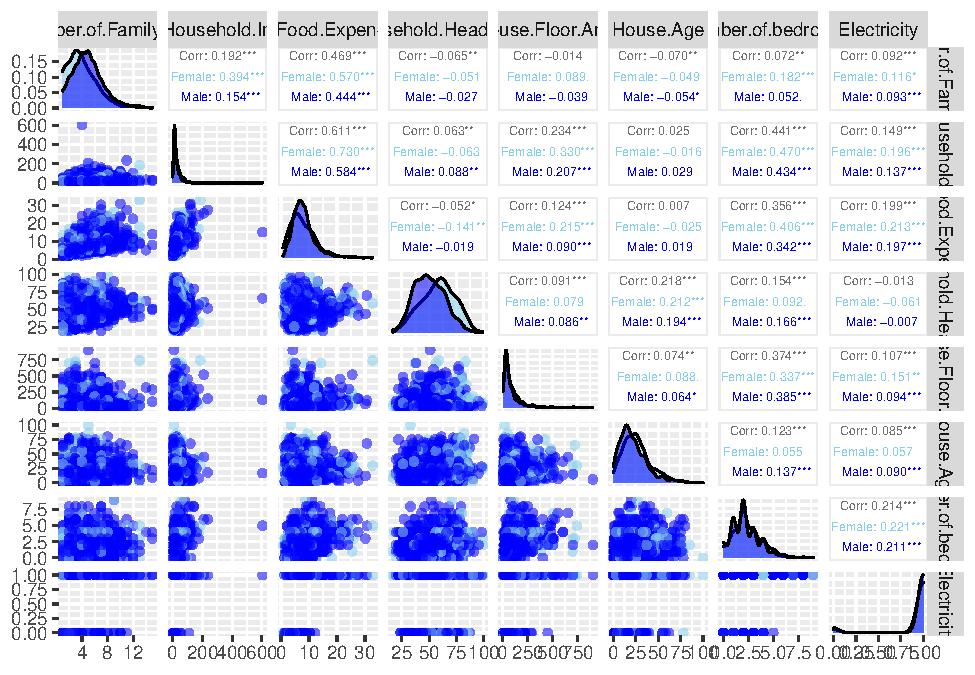
\includegraphics[width=1\linewidth]{Group_01_files/figure-latex/pairs-1} 

}

\caption{Pair plots and correlation between numerical variables, colour coded to show the sex of the head of household.}\label{fig:pairs}
\end{figure}

\begin{center}\rule{0.5\linewidth}{0.5pt}\end{center}

\newpage

\hypertarget{sec:ARC}{%
\section{Analysis of Relationships between Covariates}\label{sec:ARC}}

\hypertarget{the-relationship-between-independent-and-dependent-variables}{%
\subsection{The relationship between independent and dependent
variables}\label{the-relationship-between-independent-and-dependent-variables}}

We will explore whether nine variables related to households in the
dataset have an impact on the number of people living in the house
(Total.Number.of.Family.members). These nine variables are Annual
household income, Annual expenditure by the household on food, Head of
the household's sex, Head of the household's age, Type of Household,
Floor area of the house, Age of the building, Number of bedrooms in the
house and the presence or absence of an electricity supply to the house.

Figure 4 displays scatterplots and boxplots of the response variable
versus the explanatory variables.

\begin{figure}

{\centering 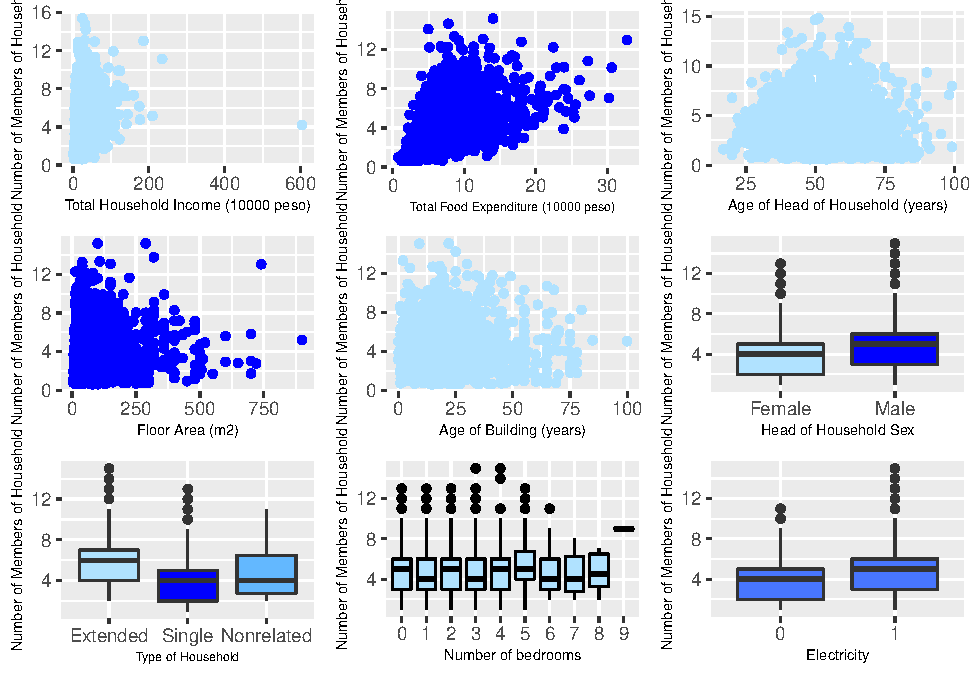
\includegraphics[width=1\linewidth]{Group_01_files/figure-latex/single predictor scatterplots-1} 

}

\caption{Scatterplots and Boxplots of each predictor against the response variable}\label{fig:single predictor scatterplots}
\end{figure}

From Figure 4, it can be seen that total food expenditure (in 10000
peso), age of the head of household, sex of the head of household and
age of the house seem to have a weak effect on the number of people in
the household. However, we will analyze the details below by GLM.

\hypertarget{gender-age}{%
\subsection{Gender \& Age}\label{gender-age}}

As highlighted by the pairs plot in Figure 3, there appears to be a
relationship between the sex and age of the head of the household.

The minimum and maximum ages of household heads do not appear to differ
greatly according to the individuals' sex, however they do differ at the
25th, 50th and 75th percentiles with male heads of households being
consitently younger than their female counterparts. The standard
deviation is also greater for the female group, but the substantially
smaller group size for females may contribute to this larger variation.

\begin{table}[!h]

\caption{\label{tab:summaries of age by sex}Summary statistics on the age of household heads by sex.}
\centering
\begin{tabular}[t]{l|r|r|r|r|r|r|r|r}
\hline
Household.Head.Sex & n & Mean & St.Dev & Min & Q1 & Median & Q3 & Max\\
\hline
Female & 369 & 58.23 & 15.69 & 17 & 47 & 59 & 69 & 99\\
\hline
Male & 1356 & 50.59 & 13.74 & 20 & 40 & 49 & 61 & 98\\
\hline
\end{tabular}
\end{table}

The boxplot in Figure 5 illustrates the previously summarised data. The
boxplot identifies the two oldest male head of households as outliers
(shown by the points above the whisker), however within the context of
the data and when compared to the ages of female head of household
boxplot, these ages do not appear unreasonable or unrealistic.

\begin{figure}

{\centering 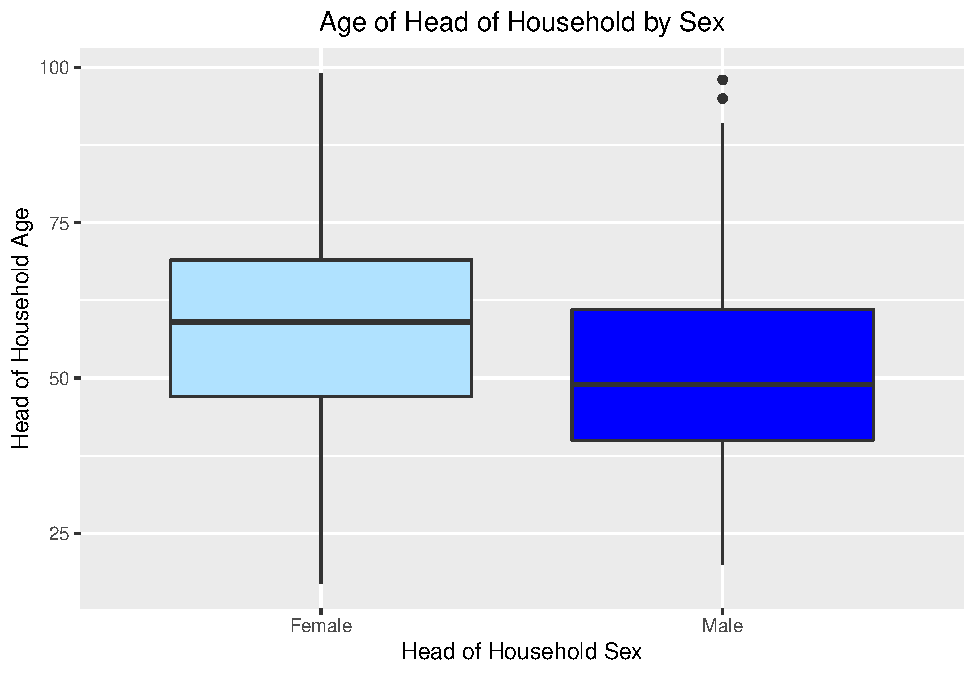
\includegraphics[width=0.8\linewidth]{Group_01_files/figure-latex/boxplot of age by gender-1} 

}

\caption{Boxplots of Head of Household Age stratified by Sex}\label{fig:boxplot of age by gender}
\end{figure}

The following Mann-Whitney U-test shows that there is a statistically
significant difference in the median ages of male and female head of
households at a 5\% level.

\begin{verbatim}
    Wilcoxon rank sum test with continuity correction

data:  data.gender$Household.Head.Age by data.gender$Household.Head.Sex
W = 324284, p-value < 2.2e-16
alternative hypothesis: true location shift is not equal to 0
\end{verbatim}

\hypertarget{household-income-and-food-expenditure}{%
\subsection{Household Income and Food
Expenditure}\label{household-income-and-food-expenditure}}

Figure 6 shows a boxplot of household incomes suggests a heavily skewed
distribution with many outliers at the upper end of the distribution.

\begin{figure}[H]

{\centering 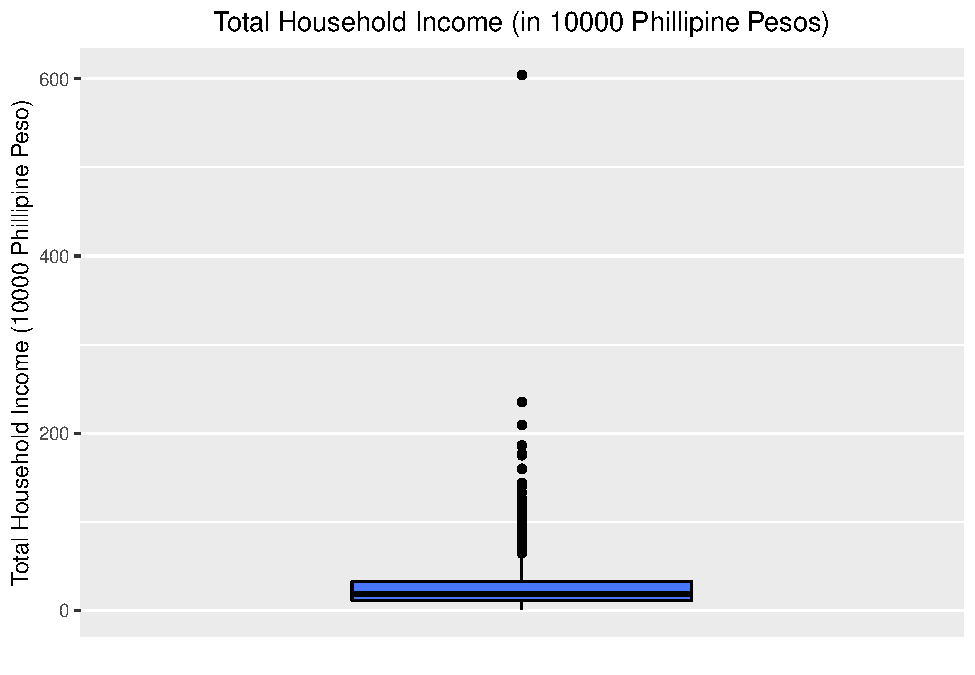
\includegraphics[width=0.8\linewidth]{Group_01_files/figure-latex/balance boxplot-1} 

}

\caption{Household Incomes in 10000 Phillipine Pesos.}\label{fig:balance boxplot}
\end{figure}

The boxplot in Figure 7 shows the log transformed household income and
shows there are still several outliers following the transformation.

\begin{figure}[H]

{\centering 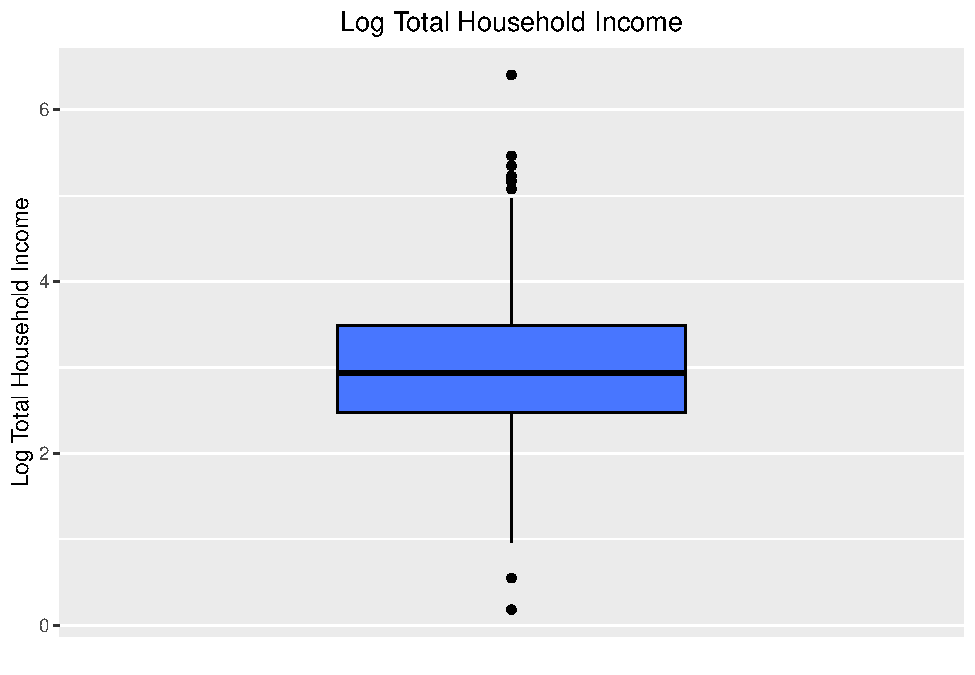
\includegraphics[width=0.8\linewidth]{Group_01_files/figure-latex/balance boxplot2-1} 

}

\caption{Boxplot of log transformed Incomes.}\label{fig:balance boxplot2}
\end{figure}

The scatterplot in Figure 8 of total household income against total food
expenditure suggests a moderate positive correlation but the fitted
model may be being heavily influenced by the extreme values,
particularly by one extreme point.

\begin{figure}[H]

{\centering 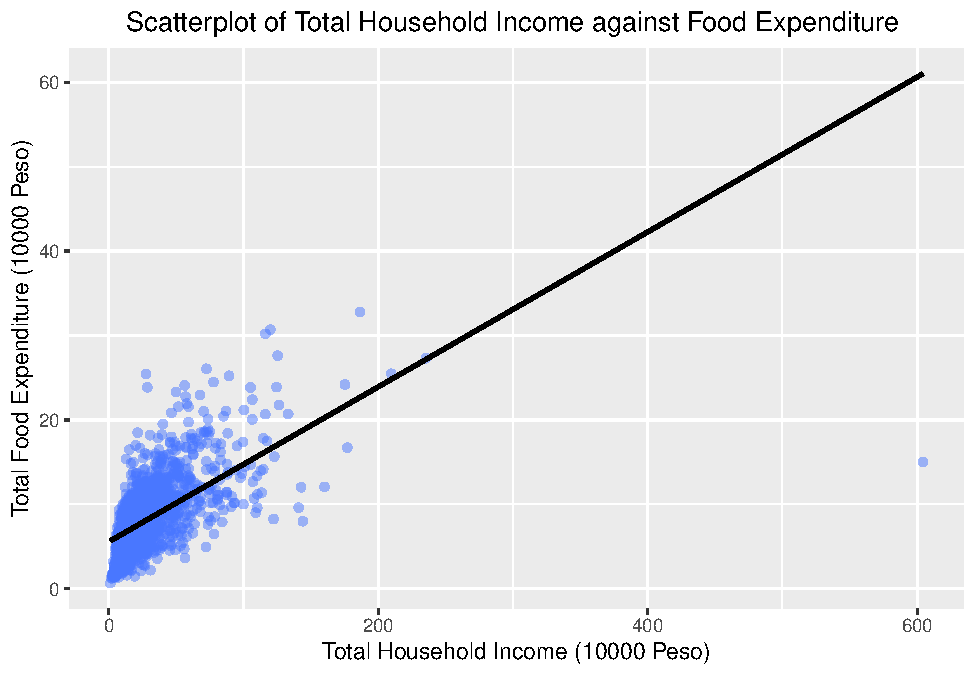
\includegraphics[width=0.8\linewidth]{Group_01_files/figure-latex/balance_plot-1} 

}

\caption{Scatterplot of Income against Food Expenditure.}\label{fig:balance_plot}
\end{figure}

Figure 8 again highlights a possible outlier in terms of income, this
could be a data entry error or just an outlier at the maximum. Removing
this observation from the data set and plotting provides the following
scatter diagram in Figure 10. This plot reconfirms the suggested
positive correlation, but there is still an imbalance in the amount of
data available at different levels of income. For example, most data is
available for incomes between 0 and 750000 peso, but far fewer data
points occur above this income level.

\begin{figure}[H]

{\centering 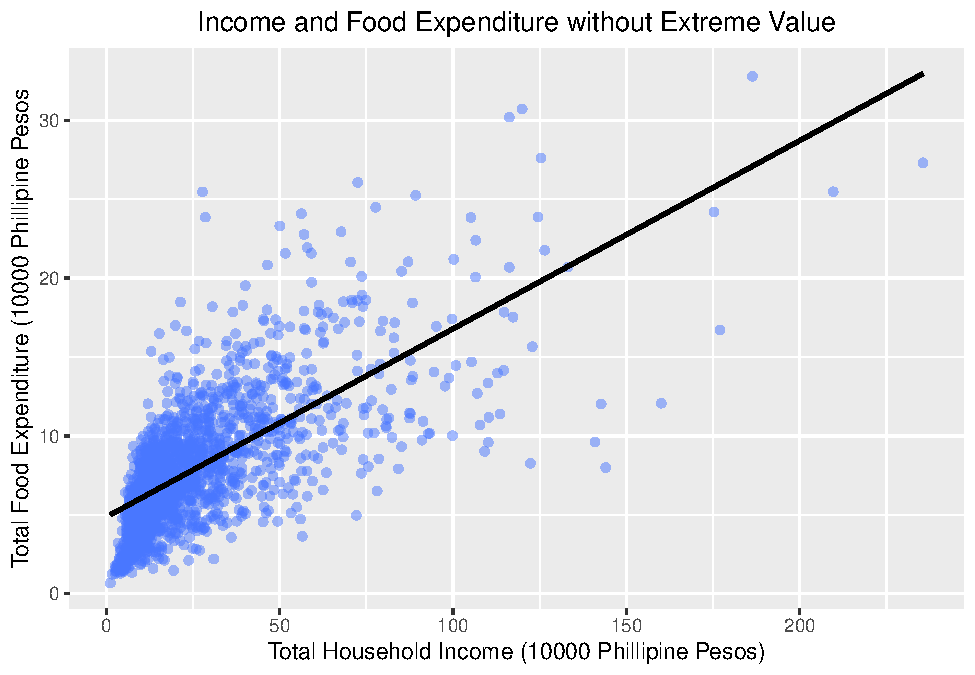
\includegraphics[width=0.8\linewidth]{Group_01_files/figure-latex/balance without outlier-1} 

}

\caption{Scatterplot of Income and Food Expenditure with extreme value removed.}\label{fig:balance without outlier}
\end{figure}

\hypertarget{number-of-family-members-head-of-household-sex}{%
\subsection{Number of Family Members \& Head of Household
Sex}\label{number-of-family-members-head-of-household-sex}}

\begin{figure}[H]

{\centering 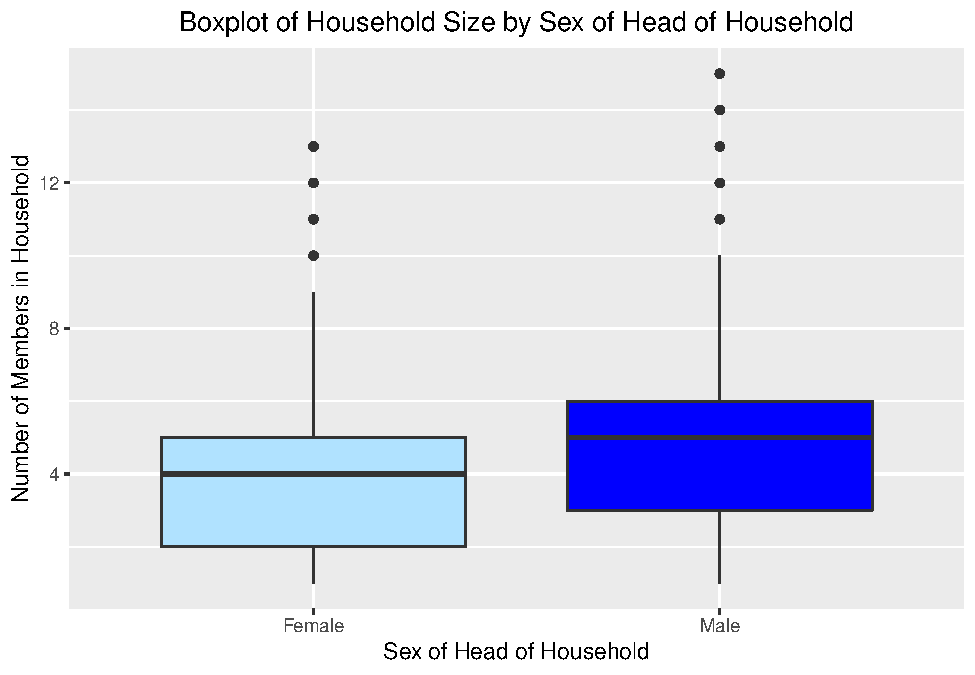
\includegraphics[width=0.8\linewidth]{Group_01_files/figure-latex/boxplot of sex and members-1} 

}

\caption{Number of Members in Household by Sex of Head of Household}\label{fig:boxplot of sex and members}
\end{figure}

Hence we can see from Figure 10 that households with a male head appear
to have a greater number of family members on average than those with a
female head, as the male group has larger values for the first and third
quartiles and the median. However there is overlap between the two
groups central IQR and so the distributions may not be significantly
different.

Figure 11 shows that an extended family household or one formed by
non-related individuals is more likely to have a female head, whereas a
larger proportion of single family households have male heads.

\begin{figure}[H]

{\centering 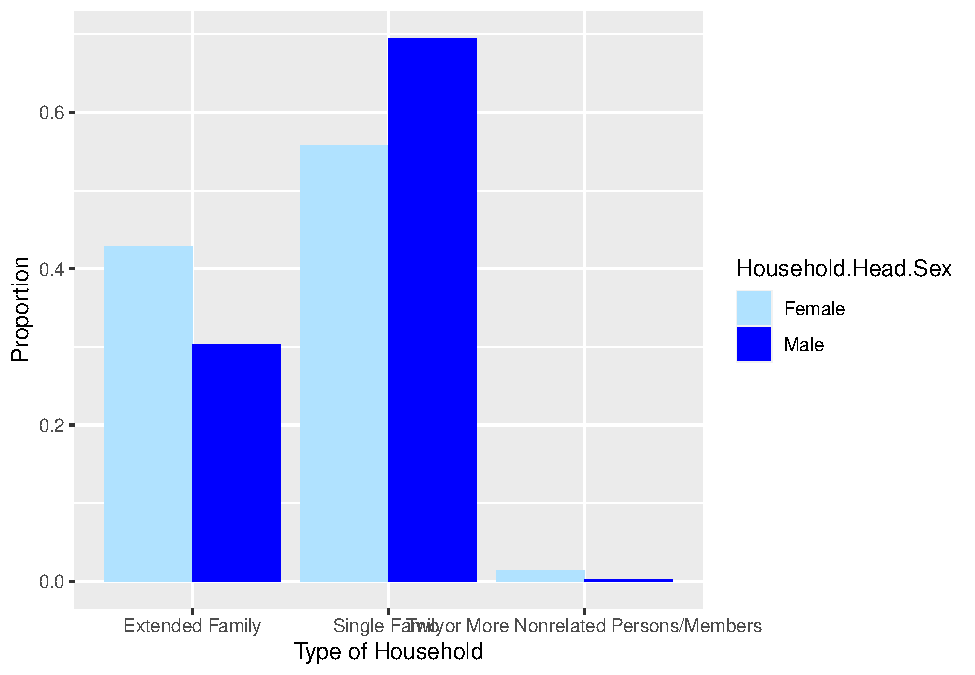
\includegraphics[width=0.8\linewidth]{Group_01_files/figure-latex/barplot of sex by type of household-1} 

}

\caption{Barplot of household head's sex by type of household}\label{fig:barplot of sex by type of household}
\end{figure}

\begin{center}\rule{0.5\linewidth}{0.5pt}\end{center}

\newpage

\hypertarget{sec:EMA}{%
\section{Exploratory Model Analysis}\label{sec:EMA}}

\hypertarget{glm-model-exploration}{%
\subsection{GLM Model Exploration}\label{glm-model-exploration}}

Prior to exploring any models, the outlier for Total Household Income
and corresponding measurements for the other variables from this
individual are removed.

The following code identifies which explanatory variables would be
included to produce the best models of different sizes, in this instance
the maximum number of variables specified is ten. The output suggests
the first predictor to be included is the total food expenditure in
10000 Philippine pesos, and the last to be included is the binary
variable Electricity that identifies if a household has electricity.
Comparing each of the ten models produced by BIC, CP and adjusted R\^{}2
selection criteria is inconclusive as each implies a different model is
best.

\begin{verbatim}
Subset selection object
Call: regsubsets.formula(Total.Number.of.Family.members ~ ., data = data, 
    nvmax = 10)
10 Variables  (and intercept)
                                                        Forced in Forced out
Total.Household.Income                                      FALSE      FALSE
Total.Food.Expenditure                                      FALSE      FALSE
Household.Head.SexMale                                      FALSE      FALSE
Household.Head.Age                                          FALSE      FALSE
Type.of.HouseholdSingle Family                              FALSE      FALSE
Type.of.HouseholdTwo or More Nonrelated Persons/Members     FALSE      FALSE
House.Floor.Area                                            FALSE      FALSE
House.Age                                                   FALSE      FALSE
Number.of.bedrooms                                          FALSE      FALSE
Electricity                                                 FALSE      FALSE
1 subsets of each size up to 10
Selection Algorithm: exhaustive
          Total.Household.Income Total.Food.Expenditure Household.Head.SexMale
1  ( 1 )  " "                    "*"                    " "                   
2  ( 1 )  " "                    "*"                    " "                   
3  ( 1 )  " "                    "*"                    "*"                   
4  ( 1 )  "*"                    "*"                    "*"                   
5  ( 1 )  "*"                    "*"                    "*"                   
6  ( 1 )  "*"                    "*"                    "*"                   
7  ( 1 )  "*"                    "*"                    "*"                   
8  ( 1 )  "*"                    "*"                    "*"                   
9  ( 1 )  "*"                    "*"                    "*"                   
10  ( 1 ) "*"                    "*"                    "*"                   
          Household.Head.Age Type.of.HouseholdSingle Family
1  ( 1 )  " "                " "                           
2  ( 1 )  " "                "*"                           
3  ( 1 )  " "                "*"                           
4  ( 1 )  " "                "*"                           
5  ( 1 )  " "                "*"                           
6  ( 1 )  " "                "*"                           
7  ( 1 )  "*"                "*"                           
8  ( 1 )  "*"                "*"                           
9  ( 1 )  "*"                "*"                           
10  ( 1 ) "*"                "*"                           
          Type.of.HouseholdTwo or More Nonrelated Persons/Members
1  ( 1 )  " "                                                    
2  ( 1 )  " "                                                    
3  ( 1 )  " "                                                    
4  ( 1 )  " "                                                    
5  ( 1 )  " "                                                    
6  ( 1 )  " "                                                    
7  ( 1 )  " "                                                    
8  ( 1 )  " "                                                    
9  ( 1 )  "*"                                                    
10  ( 1 ) "*"                                                    
          House.Floor.Area House.Age Number.of.bedrooms Electricity
1  ( 1 )  " "              " "       " "                " "        
2  ( 1 )  " "              " "       " "                " "        
3  ( 1 )  " "              " "       " "                " "        
4  ( 1 )  " "              " "       " "                " "        
5  ( 1 )  " "              "*"       " "                " "        
6  ( 1 )  " "              "*"       "*"                " "        
7  ( 1 )  " "              "*"       "*"                " "        
8  ( 1 )  "*"              "*"       "*"                " "        
9  ( 1 )  "*"              "*"       "*"                " "        
10  ( 1 ) "*"              "*"       "*"                "*"        
\end{verbatim}

\begin{verbatim}
Adj.R2     CP    BIC 
     9      8      6 
\end{verbatim}

\begin{center}\rule{0.5\linewidth}{0.5pt}\end{center}

\newpage

\hypertarget{sec:FMA}{%
\section{Formal Model Analysis}\label{sec:FMA}}

\hypertarget{poisson-regression-model}{%
\subsection{Poisson Regression model}\label{poisson-regression-model}}

The response variable of the Total Number of Family Members (or members
of the household) can be viewed as a count and therefore a Poisson
Regression model is considered. For a Poisson model to be suitable, the
mean and variance should be equal and so these assumptions are checked
first.

\begin{table}

\caption{\label{tab:poisson mean and variance check}Mean and Variation of Response Variable}
\centering
\begin{tabular}[t]{l|r}
\hline
  & \\
\hline
Mean & 4.669373\\
\hline
Variance & 5.446049\\
\hline
\end{tabular}
\end{table}

From Table 5, we see the variation of total number of family members is
only marginally larger than the mean of total number of family members,
thus, the possibility of over-dispersion in our model is not a
significant issue.

\begin{table}[!h]
\centering
\begin{tabular}{lr}
\toprule
\cellcolor{gray!6}{Observations} & \cellcolor{gray!6}{1724}\\
Dependent variable & Total.Number.of.Family.members\\
\cellcolor{gray!6}{Type} & \cellcolor{gray!6}{Generalized linear model}\\
Family & poisson\\
\cellcolor{gray!6}{Link} & \cellcolor{gray!6}{log}\\
\bottomrule
\end{tabular}
\end{table} \begin{table}[!h]
\centering
\begin{tabular}{lr}
\toprule
\cellcolor{gray!6}{$\chi^2$(10)} & \cellcolor{gray!6}{693.90}\\
Pseudo-R² (Cragg-Uhler) & 0.34\\
\cellcolor{gray!6}{Pseudo-R² (McFadden)} & \cellcolor{gray!6}{0.09}\\
AIC & 7011.64\\
\cellcolor{gray!6}{BIC} & \cellcolor{gray!6}{7071.61}\\
\bottomrule
\end{tabular}
\end{table} \begin{table}[!h]
\centering
\begin{threeparttable}
\begin{tabular}{lrrrr}
\toprule
  & Est. & S.E. & z val. & p\\
\midrule
\cellcolor{gray!6}{(Intercept)} & \cellcolor{gray!6}{1.43} & \cellcolor{gray!6}{0.08} & \cellcolor{gray!6}{17.90} & \cellcolor{gray!6}{0.00}\\
Total.Household.Income & -0.00 & 0.00 & -3.33 & 0.00\\
\cellcolor{gray!6}{Total.Food.Expenditure} & \cellcolor{gray!6}{0.05} & \cellcolor{gray!6}{0.00} & \cellcolor{gray!6}{14.08} & \cellcolor{gray!6}{0.00}\\
Household.Head.Age & -0.00 & 0.00 & -2.89 & 0.00\\
\cellcolor{gray!6}{House.Floor.Area} & \cellcolor{gray!6}{-0.00} & \cellcolor{gray!6}{0.00} & \cellcolor{gray!6}{-1.51} & \cellcolor{gray!6}{0.13}\\
\addlinespace
House.Age & -0.00 & 0.00 & -3.00 & 0.00\\
\cellcolor{gray!6}{Number.of.bedrooms} & \cellcolor{gray!6}{-0.01} & \cellcolor{gray!6}{0.01} & \cellcolor{gray!6}{-1.53} & \cellcolor{gray!6}{0.13}\\
Electricity & 0.03 & 0.05 & 0.58 & 0.56\\
\cellcolor{gray!6}{Household.Head.SexMale} & \cellcolor{gray!6}{0.22} & \cellcolor{gray!6}{0.03} & \cellcolor{gray!6}{7.41} & \cellcolor{gray!6}{0.00}\\
Type.of.HouseholdSingle Family & -0.35 & 0.02 & -14.04 & 0.00\\
\addlinespace
\cellcolor{gray!6}{Type.of.HouseholdTwo or More Nonrelated Persons/Members} & \cellcolor{gray!6}{-0.14} & \cellcolor{gray!6}{0.16} & \cellcolor{gray!6}{-0.90} & \cellcolor{gray!6}{0.37}\\
\bottomrule
\end{tabular}
\begin{tablenotes}
\item Standard errors: MLE
\end{tablenotes}
\end{threeparttable}
\end{table}

The poisson model fitted with all possible covariates concludes there
are six statistically significant predictors at the 5\% level. These are
the total household income and food expenditure, the age and gender of
the head of the household, the age of the house and if it is a single
family household. Table 6 shows the estimates and the lower and upper
bounds of the 95\% confidence intervals for the regression parameters.
The rows containing significant predictors, and so where the confidence
intervals do not include 0, are highlighted. We can clearly see that the
confidence intervals for area, number of bedrooms, and electricity
access include 0. This indicates that these three variables have
essentially no effect on the number of people in the household, which
exactly validates the results for the p-value as well.

\textbackslash begin\{table\}

\textbackslash caption\{\label{tab:table of estimates and confidence intervals}Estimates
and the corresponding 95\% Confidence Intervals, with significant
predictors highlighted.\} \centering

\begin{tabular}[t]{l|r|r|r}
\hline
  & Lower Bound & Estimate & Upper Bound\\
\hline
\cellcolor[HTML]{A1E8F1}{\textcolor{black}{(Intercept)}} & \cellcolor[HTML]{A1E8F1}{\textcolor{black}{1.2687606}} & \cellcolor[HTML]{A1E8F1}{\textcolor{black}{1.4254422}} & \cellcolor[HTML]{A1E8F1}{\textcolor{black}{1.5810043}}\\
\hline
\cellcolor[HTML]{A1E8F1}{\textcolor{black}{Total.Household.Income}} & \cellcolor[HTML]{A1E8F1}{\textcolor{black}{-0.0035110}} & \cellcolor[HTML]{A1E8F1}{\textcolor{black}{-0.0022045}} & \cellcolor[HTML]{A1E8F1}{\textcolor{black}{-0.0009192}}\\
\hline
\cellcolor[HTML]{A1E8F1}{\textcolor{black}{Total.Food.Expenditure}} & \cellcolor[HTML]{A1E8F1}{\textcolor{black}{0.0430507}} & \cellcolor[HTML]{A1E8F1}{\textcolor{black}{0.0500316}} & \cellcolor[HTML]{A1E8F1}{\textcolor{black}{0.0569775}}\\
\hline
\cellcolor[HTML]{A1E8F1}{\textcolor{black}{Household.Head.Age}} & \cellcolor[HTML]{A1E8F1}{\textcolor{black}{-0.0042279}} & \cellcolor[HTML]{A1E8F1}{\textcolor{black}{-0.0025205}} & \cellcolor[HTML]{A1E8F1}{\textcolor{black}{-0.0008148}}\\
\hline
House.Floor.Area & -0.0004469 & -0.0001932 & 0.0000552\\
\hline
\cellcolor[HTML]{A1E8F1}{\textcolor{black}{House.Age}} & \cellcolor[HTML]{A1E8F1}{\textcolor{black}{-0.0038392}} & \cellcolor[HTML]{A1E8F1}{\textcolor{black}{-0.0023168}} & \cellcolor[HTML]{A1E8F1}{\textcolor{black}{-0.0008069}}\\
\hline
Number.of.bedrooms & -0.0333633 & -0.0145830 & 0.0041111\\
\hline
Electricity & -0.0644803 & 0.0276347 & 0.1219537\\
\hline
\cellcolor[HTML]{A1E8F1}{\textcolor{black}{Household.Head.SexMale}} & \cellcolor[HTML]{A1E8F1}{\textcolor{black}{0.1623556}} & \cellcolor[HTML]{A1E8F1}{\textcolor{black}{0.2202770}} & \cellcolor[HTML]{A1E8F1}{\textcolor{black}{0.2788479}}\\
\hline
\cellcolor[HTML]{A1E8F1}{\textcolor{black}{Type.of.HouseholdSingle Family}} & \cellcolor[HTML]{A1E8F1}{\textcolor{black}{-0.3967514}} & \cellcolor[HTML]{A1E8F1}{\textcolor{black}{-0.3481835}} & \cellcolor[HTML]{A1E8F1}{\textcolor{black}{-0.2995260}}\\
\hline
Type.of.HouseholdTwo or More Nonrelated Persons/Members & -0.4743426 & -0.1444455 & 0.1540719\\
\hline
\end{tabular}

\textbackslash end\{table\}

We refit the model to include just the previously identified significant
covariates and again evaluated the 95\% confidence intervals for the
estimated parameters, these values can be seen in Table 7. The intercept
term of 1.436 is simply a positional constant due to the context of the
variables. The negative coefficient of Total Household Income shows that
for every additional 10000 peso, the number of household members is
expected to decrease by 0.002. The coefficient of Total Food Expenditure
suggests that for an increase of 10000 peso in spending, there is an
expected 0.048 more members in the household. The coefficients of Head
of Household age and the Age of the Building are both negative (-0.003
and -0.002 respectively) showing that an older head of the household or
older building is linked to fewer members in a household. A Single
Family household is expected to have 0.350 fewer members than the
baseline category of an extended family household, and households with a
male head will have 0.222 members more than their female counterparts.

\begin{table}[!h]
\centering
\begin{tabular}{lr}
\toprule
\cellcolor{gray!6}{Observations} & \cellcolor{gray!6}{1724}\\
Dependent variable & Total.Number.of.Family.members\\
\cellcolor{gray!6}{Type} & \cellcolor{gray!6}{Generalized linear model}\\
Family & poisson\\
\cellcolor{gray!6}{Link} & \cellcolor{gray!6}{log}\\
\bottomrule
\end{tabular}
\end{table} \begin{table}[!h]
\centering
\begin{tabular}{lr}
\toprule
\cellcolor{gray!6}{$\chi^2$(7)} & \cellcolor{gray!6}{687.54}\\
Pseudo-R² (Cragg-Uhler) & 0.33\\
\cellcolor{gray!6}{Pseudo-R² (McFadden)} & \cellcolor{gray!6}{0.09}\\
AIC & 7012.00\\
\cellcolor{gray!6}{BIC} & \cellcolor{gray!6}{7055.62}\\
\bottomrule
\end{tabular}
\end{table} \begin{table}[!h]
\centering
\begin{threeparttable}
\begin{tabular}{lrrrr}
\toprule
  & Est. & S.E. & z val. & p\\
\midrule
\cellcolor{gray!6}{(Intercept)} & \cellcolor{gray!6}{1.43} & \cellcolor{gray!6}{0.07} & \cellcolor{gray!6}{21.27} & \cellcolor{gray!6}{0.00}\\
Total.Household.Income & -0.00 & 0.00 & -4.59 & 0.00\\
\cellcolor{gray!6}{Total.Food.Expenditure} & \cellcolor{gray!6}{0.05} & \cellcolor{gray!6}{0.00} & \cellcolor{gray!6}{14.29} & \cellcolor{gray!6}{0.00}\\
Household.Head.Age & -0.00 & 0.00 & -3.21 & 0.00\\
\cellcolor{gray!6}{House.Age} & \cellcolor{gray!6}{-0.00} & \cellcolor{gray!6}{0.00} & \cellcolor{gray!6}{-3.23} & \cellcolor{gray!6}{0.00}\\
\addlinespace
Household.Head.SexMale & 0.22 & 0.03 & 7.42 & 0.00\\
\cellcolor{gray!6}{Type.of.HouseholdSingle Family} & \cellcolor{gray!6}{-0.35} & \cellcolor{gray!6}{0.02} & \cellcolor{gray!6}{-14.08} & \cellcolor{gray!6}{0.00}\\
Type.of.HouseholdTwo or More Nonrelated Persons/Members & -0.14 & 0.16 & -0.85 & 0.39\\
\bottomrule
\end{tabular}
\begin{tablenotes}
\item Standard errors: MLE
\end{tablenotes}
\end{threeparttable}
\end{table}

It is important to note that the p-value for Family type of two or more
unrelated individuals is greater than 0.05, thus indicating that a
family type of two or more nonrelated persons is not a statistically
significant explanatory variable, but households composed of a single
family (p value \textless0.05) is a statistically significant predictor
for the number of members of a household.

\textbackslash begin\{table\}

\textbackslash caption\{\label{tab:table of estimates and confidence intervals sig}Estimates
of regression parameters and the corresponding 95\% Confidence
Intervals\} \centering

\begin{tabular}[t]{l|r|r|r}
\hline
  & Lower Bound & Estimate & Upper Bound\\
\hline
\cellcolor[HTML]{A1E8F1}{\textcolor{black}{(Intercept)}} & \cellcolor[HTML]{A1E8F1}{\textcolor{black}{1.2992842}} & \cellcolor[HTML]{A1E8F1}{\textcolor{black}{1.4313832}} & \cellcolor[HTML]{A1E8F1}{\textcolor{black}{1.5630233}}\\
\hline
\cellcolor[HTML]{A1E8F1}{\textcolor{black}{Total.Household.Income}} & \cellcolor[HTML]{A1E8F1}{\textcolor{black}{-0.0040352}} & \cellcolor[HTML]{A1E8F1}{\textcolor{black}{-0.0028211}} & \cellcolor[HTML]{A1E8F1}{\textcolor{black}{-0.0016258}}\\
\hline
\cellcolor[HTML]{A1E8F1}{\textcolor{black}{Total.Food.Expenditure}} & \cellcolor[HTML]{A1E8F1}{\textcolor{black}{0.0434480}} & \cellcolor[HTML]{A1E8F1}{\textcolor{black}{0.0503772}} & \cellcolor[HTML]{A1E8F1}{\textcolor{black}{0.0572714}}\\
\hline
\cellcolor[HTML]{A1E8F1}{\textcolor{black}{Household.Head.Age}} & \cellcolor[HTML]{A1E8F1}{\textcolor{black}{-0.0044639}} & \cellcolor[HTML]{A1E8F1}{\textcolor{black}{-0.0027721}} & \cellcolor[HTML]{A1E8F1}{\textcolor{black}{-0.0010820}}\\
\hline
\cellcolor[HTML]{A1E8F1}{\textcolor{black}{House.Age}} & \cellcolor[HTML]{A1E8F1}{\textcolor{black}{-0.0039924}} & \cellcolor[HTML]{A1E8F1}{\textcolor{black}{-0.0024807}} & \cellcolor[HTML]{A1E8F1}{\textcolor{black}{-0.0009811}}\\
\hline
\cellcolor[HTML]{A1E8F1}{\textcolor{black}{Household.Head.SexMale}} & \cellcolor[HTML]{A1E8F1}{\textcolor{black}{0.1626469}} & \cellcolor[HTML]{A1E8F1}{\textcolor{black}{0.2205681}} & \cellcolor[HTML]{A1E8F1}{\textcolor{black}{0.2791383}}\\
\hline
\cellcolor[HTML]{A1E8F1}{\textcolor{black}{Type.of.HouseholdSingle Family}} & \cellcolor[HTML]{A1E8F1}{\textcolor{black}{-0.3969151}} & \cellcolor[HTML]{A1E8F1}{\textcolor{black}{-0.3484617}} & \cellcolor[HTML]{A1E8F1}{\textcolor{black}{-0.2999140}}\\
\hline
Type.of.HouseholdTwo or More Nonrelated Persons/Members & -0.4663624 & -0.1365104 & 0.1619512\\
\hline
\end{tabular}

\textbackslash end\{table\}

The regression parameter estimates and the corresponding 95\% confidence
intervals are presented in Figure 12 for both the full Poisson Model and
the Significant Factors Poisson Model.

\begin{figure}[H]

{\centering 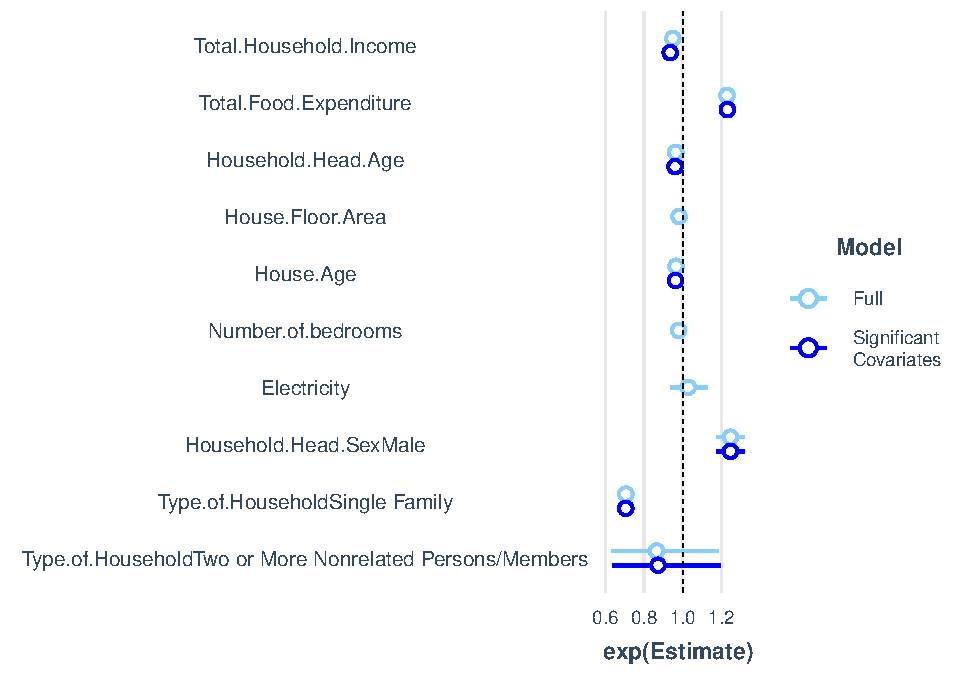
\includegraphics[width=0.8\linewidth]{Group_01_files/figure-latex/summary plot-1} 

}

\caption{Summary of Coefficients for each fitted Poisson Model}\label{fig:summary plot}
\end{figure}

\begin{longtable}[]{@{}lrr@{}}
\caption{Comparison of Fitted Poisson Models}\tabularnewline
\toprule
Model & AIC & BIC \\
\midrule
\endfirsthead
\toprule
Model & AIC & BIC \\
\midrule
\endhead
Full Model & 7011.64 & 7071.61 \\
Significant Factors Model & 7012.00 & 7055.62 \\
\bottomrule
\end{longtable}

From table 8, we find the AIC value of two fitted poisson models are
very similar, however, the BIC value for the significant factors model
is lower and so we accept the significant factors model as the better
fit for the data.

The poisson regression model that will be fitted to the data is as
follows:
\[log(\tilde{\lambda_i}) = \alpha + \beta_1 x_{1i} + \beta_2 x_{2i} + \beta_3 x_{3i} + \beta_4 x_{4i} + \widehat{\beta}_{\mbox{M}} \cdot \mathbb{I}_{\mbox{M}}(i)+\widehat{\beta}_{\mbox{S}} \cdot \mathbb{I}_{\mbox{S}}(i) + \epsilon_i, ~~~~ \epsilon \sim N(0, \sigma^2),\]
where

\begin{itemize}
\tightlist
\item
  \(log(\tilde{\lambda_i})\) is the Logged Total Number of Household
  Members of the \(i^{th}\) household;
\item
  \(x_{1i}\) is the Total Household Income in 10000 Philippine pesos of
  the \(i^{th}\) household;
\item
  \(x_{2i}\) is the Total Food Expenditure in 10000 Philippine pesos of
  the \(i^{th}\) household;
\item
  \(x_{3i}\) is the Household Head's Age in years of the \(i^{th}\)
  household;
\item
  \(x_{4i}\) is the Building Age in years of the \(i^{th}\) household;
\item
  \(\alpha\) is the intercept and positions the best-fitting plane in 3D
  space;
\item
  \(\beta_1\) is the coefficient for the first explanatory variable
  \(x_1\);
\item
  \(\beta_2\) is the coefficient for the second explanatory variable
  \(x_2\);
\item
  \(\beta_3\) is the coefficient for the third explanatory variable
  \(x_3\);
\item
  \(\beta_4\) is the coefficient for the fourth explanatory variable
  \(x_4\);
\item
  \(\widehat{\beta}_{\mbox{M}}\) is the difference in the mean total
  number of household members in a household with a male head relative
  to a female head;
\item
  \(\widehat{\beta}_{\mbox{S}}\) is the difference in the mean total
  number of household members in a household with Extended Family
  relative to Single Family;
\item
  \(\epsilon_i\) is the \(i^{th}\) random error component; and
\item
  \(\mathbb{I}_{\mbox{M}}(i)\) is an indicator function such that
\end{itemize}

\[\mathbb{I}_{\mbox{M}}(i)=\left\{
\begin{array}{ll}
1 ~~~ \mbox{if the household head of} ~ i \mbox{th observation is Male},\\
0 ~~~ \mbox{Otherwise}.\\
\end{array}
\right.\]

\begin{itemize}
\tightlist
\item
  \(\mathbb{I}_{\mbox{S}}(i)\) is an indicator function such that
\end{itemize}

\[\mathbb{I}_{\mbox{S}}(i)=\left\{
\begin{array}{ll}
1 ~~~ \mbox{if the type of household of} ~ i \mbox{th observation is Single Family},\\
0 ~~~ \mbox{Otherwise}.\\
\end{array}
\right.\]

\begin{figure}[H]

{\centering 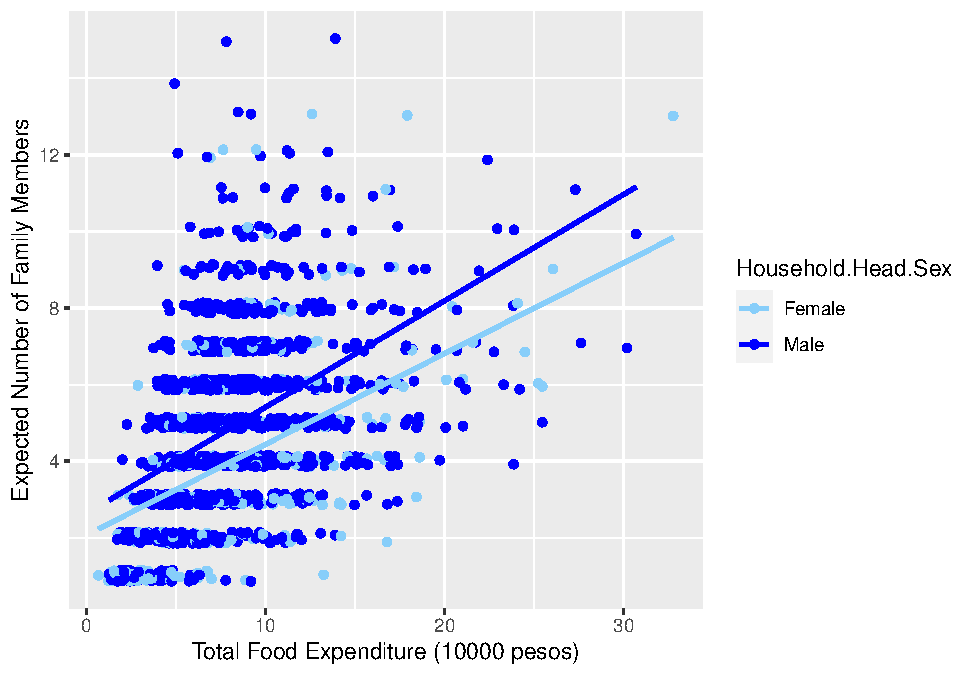
\includegraphics[width=0.8\linewidth]{Group_01_files/figure-latex/pred plot-1} 

}

\caption{Predicted Numbers of Household Members and Food Expenditure}\label{fig:pred plot}
\end{figure}

Figure 13 and Figure 14 show the expected, and observed, number of
household members plotted against the covariate Total Food Expenditure,
respectively. The fitted model lines of regression for the male and
female groups can also be seen on these plots. For Figure 14, the two
fitted lines can be seen to diverge as Food Expenditure increases,
whereas in Figure 15, the two fitted lines can be seen converging as
Food Expenditure, suggesting that the predicted model and hence
predicted data could be improved upon.

\begin{figure}[H]

{\centering 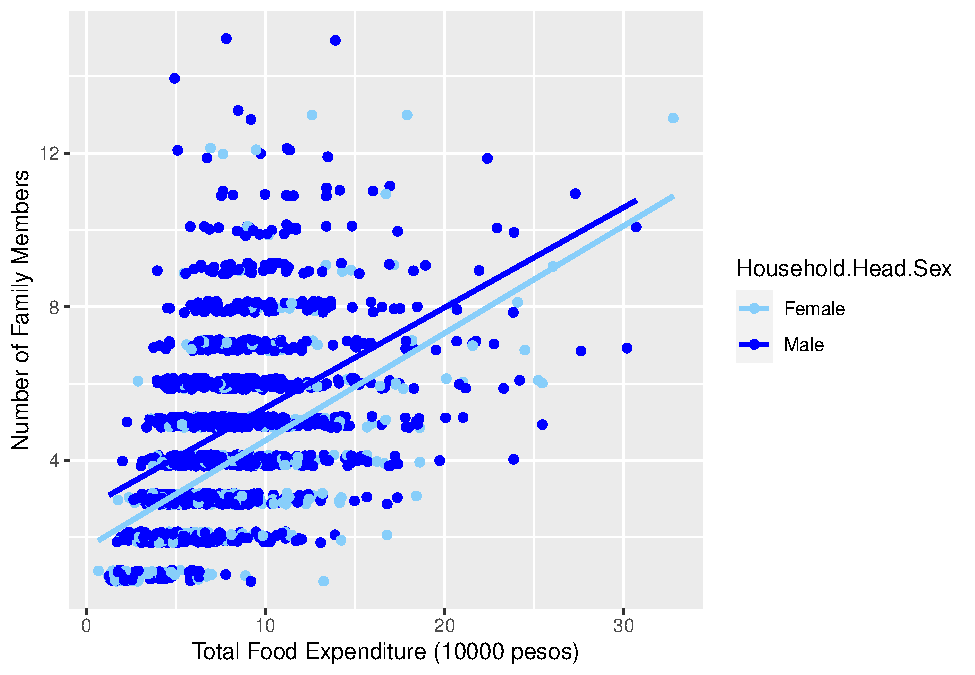
\includegraphics[width=0.8\linewidth]{Group_01_files/figure-latex/comp plot-1} 

}

\caption{Observed Numbers of Household Members and Food Expenditure}\label{fig:comp plot}
\end{figure}

Figure 15 shows the observed number of household members against the
expected number of household members, there is a definite moderate
positive correlation between these variables but it is not a perfect
correlation. This suggests the model may be improved upon, which is an
area for further analysis.

\begin{figure}[H]

{\centering 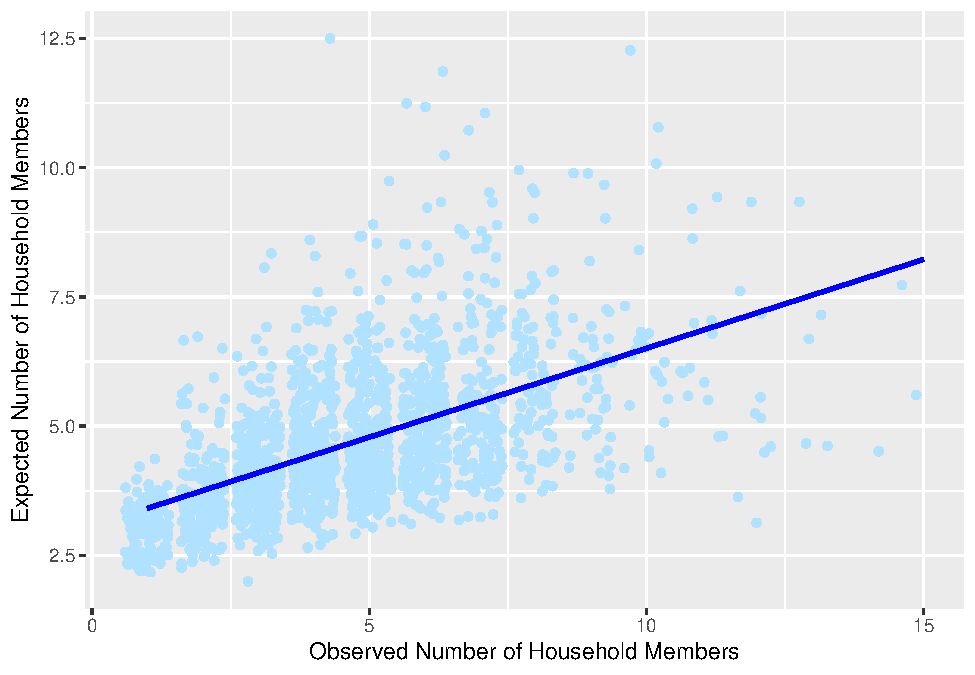
\includegraphics[width=0.8\linewidth]{Group_01_files/figure-latex/pred vs obs-1} 

}

\caption{Predicted Numbers of Household Members against Observed Number of Household Members}\label{fig:pred vs obs}
\end{figure}

\hypertarget{sec:Conc}{%
\section{Conclusions}\label{sec:Conc}}

Combining the p-values and confidence intervals for each variable, we
can conclude that Total Household Income, Total Food Expenditure, Head
of Household Age and Sex, Age of the House, and if the Household is a
Single or Extended Family, all have an effect on the number of members
in a household.

\begin{center}\rule{0.5\linewidth}{0.5pt}\end{center}

\end{document}
